\documentclass{article}
\usepackage[utf8]{inputenc}

\newcommand{\nirpdftitle}{The Sato--Tate Conjecture}
\usepackage{import}
\inputfrom{../../notes}{nir}
\usepackage[backend=biber,
    style=alphabetic,
    sorting=ynt
]{biblatex}
\setcounter{tocdepth}{2}

\pagestyle{contentpage}

\title{The Sato--Tate Conjecture}
\author{Nir Elber}
\date{Fall 2024}
\usepackage{graphicx}

\begin{document}

\maketitle

\begin{abstract}
	This is an expository note for two talks on the Sato--Tate conjecture. In the first talk, we will state the Sato--Tate conjecture for abelian varieties. In the second talk, we will discuss some results related to Sato--Tate groups of the so-called Fermat curves $x^m+y^m+z^m=0$.
\end{abstract}

\tableofcontents

\section{Stating the Sato--Tate Conjecture}
In this first talk, we will work our way towards stating the Sato--Tate conjecture for abelian varieties. We will gradually increase the amount of assumed background.

\subsection{Quadratic Equations}
In order to get a dishonest taste for the sort of results we are after, we will begin with the case of quadratic equations. Fix a monic quadratic polynomial $f(x)=x^2+ax+b$ with nonzero discriminant $a^2-4b$, and consider the curve
\[C\colon y^2=f(x).\]
Technically speaking, we understand $C_f$ to cut out a smooth projective curve in $\PP^2_\QQ$ given by homogenizing.
\begin{example}
	For this section, it will be enough to follow the example $C\colon y^2=x^2+1$ around. The polynomial $x^2+1$ has discriminant $-4$.
\end{example}
Because this is a talk about arithmetic geometry, we are interested in the number of points on $C_f$. Studying points over $\QQ$ or $\ZZ$ is rather difficult (and will continue to get harder when we change the curve later), so we will content ourselves with studying the number of points over finite fields. Even though our curve is a priori defined over $\QQ$, we see that $f(x)\in\ZZ[x]$ allows us to give $C_f$ a model over $\ZZ$ given by the same equation. In this way, we can formally make sense of $C(\FF_q)$ for any finite field $\FF_q$.
\begin{remark}
	In practice, one can think about $C(\FF_q)$ as the number of pairs $(x,y)\in\FF_q^2$ satisfying the equation given by $C$. The above process of finding an integral model should be thought of as some formal general procedure.
\end{remark}
\begin{remark}
	Our choice of integral model may not always make sense at all primes $p$. Notably, we would like for $C_f$ to define a smooth curve over $\FF_p$, but this requires $a^2-4b\ne0$ (for example). (For odd primes $p$, smoothness is equivalent to $a^2-4b\ne0$.) Over $\QQ$, this was a hypothesis, but in general, $a^2-4b$ can vanish$\pmod p$ for some primes $p$. For example, $y^2=x^2+1$ fails to be smooth over $\FF_2$.
\end{remark}
Let us begin with an expectation for $C(\FF_q)$. For each $x\in\FF_q$, it will be difficult to control the value of $f(x)$. However, about half of $\FF_q$ has two square roots, and about half of $\FF_q$ has no square roots, so it seems reasonably to expect that each $f(x)\in\FF_q$ has on average one square root. Thus, we may expect that
\[C(\FF_q)\approx q+1,\]
where we have added $1$ to include the point(s) at infinity. Let's see what we get.
\begin{example}
	We continue with the curve $C\colon y^2=x^2+1$. A computer program gives the following output.
	\[\begin{array}{c|ccccccccccccccccc}
		p & 3 & 5 & 7 & 11 & 13 & 17 & 19 & 23 & 29 & 31 & 37 & 41 & 43 & 47 \\\hline
		\#C(\mathbb F_p) & 4 & 6 & 8 & 12 & 14 & 18 & 20 & 24 & 30 & 32 & 38 & 42 & 44 & 48 \\
		p+1 & 4 & 6 & 8 & 12 & 14 & 18 & 20 & 24 & 30 & 32 & 38 & 42 & 44 & 48
	\end{array}\]
\end{example}
Huh, it looks like our guess was pretty spot-on.
\begin{exe}
	For a curve $C\colon y^2=x^2+d$ for some $d\in\ZZ$, show that $\#C(\FF_q)=q+1$ for any finite field $\FF_q$. You may find it helpful to use the substitution $(s,d)=(x+y,x-y)$.
\end{exe}
\begin{remark}
	Intuitively, what is going on here is that quadratics cut out genus $0$ curves, which must all be isomorphic to $\PP^1$.
\end{remark}

\subsection{Two Elliptic Curves}
Let's move on to a more nontrivial example. Most of this first talk will be interested in elliptic curves, for which we pick up the following concrete definition.
\begin{definition}[elliptic curve]
	Fix a field $K$ of characteristic not equal to $2$ or $3$. Then an \textit{elliptic curve} is a curve of the form
	\[E\colon y^2=x^3+ax+b,\]
	where $a,b\in K$, and the discriminant $-4a^3-27b^2$ is nonzero. As usual, $E$ is understood to cut out a smooth projective curve in $\PP^2_K$ given by homogeneizing to $Y^2Z=X^3+aXZ^2+bZ^3$, so there is one point $[0:1:0]$ at infinity.
\end{definition}
For today, all of our elliptic curves $E$ will be defined over $\QQ$ and pretty good integral models.
\begin{example} \label{ex:ec-as-c-mod-lattice}
	For any lattice $\Lambda\subseteq\CC$, it turns out that one can realize $\CC/\Lambda$ as an elliptic curve over $\CC$.
\end{example}
\begin{example}
	We will follow around the two elliptic curves
	\[E_1\colon y^2=x^3+1\qquad\text{and}\qquad E_2\colon y^2=x^3+x+1\]
	for this section. Though they look similar, these two curves have very different behavior!
\end{example}
As in the previous section, we note that one can frequently define a notion of $E(\FF_q)$. Namely, the cubic equation defining $E$ will only have finitely many denominators, and the discriminant of the cubic equation will only have finitely many prime factors; away from these primes, the equation defining $E$ will define a perfectly reasonable elliptic curve over $\FF_{p^r}$ for any $r\ge1$.
\begin{example}
	We discuss models for our elliptic curves $E_1$ and $E_2$. Note that their defining equations have no denominators.
	\begin{itemize}
		\item We see that $E_1\colon y^2=x^3+1$ has discriminat $-27$, so we get an elliptic curve over $\FF_{p^r}$ for any $p\ne3$.
		\item Similarly, the curve $E_2\colon y^2=x^3+x+1$ has discriminant $-31$, so we get an elliptic curve over $\FF_{p^r}$ for any $p\ne31$.
	\end{itemize}
\end{example}
Once again, for any value of $x$, there is no reason to expect $x^3+ax+b$ to be a square or not, so a reasonable expectation is for
\[E(\FF_q)\approx q+1.\]
Let's see what we get.
\begin{example}
	We continue with the two elliptic curves $E_1\colon y^2=x^3+1$ and $E_2\colon y^2=x^3+x+1$.
	\[\begin{array}{c|ccccccccccccccccc}
		p & 5 & 7 & 11 & 13 & 17 & 19 & 23 & 29 & 37 & 41 & 43 & 47 \\\hline
		\#E_1(\mathbb F_p) & 6 & 12 & 12 & 12 & 18 & 12 & 24 & 30 & 48 & 42 & 36 & 48 \\
		\#E_2(\mathbb F_p) & 9 & 5 & 14 & 18 & 18 & 21 & 28 & 36 & 48 & 35 & 34 & 60 \\
		p+1 & 6 & 8 & 12 & 14 & 18 & 20 & 24 & 30 & 38 & 42 & 44 & 48
	\end{array}\]
\end{example}
Our guess seems to be pretty close but not quite spot-on. Let's examine the error.
\begin{example}
	We continue with the two elliptic curves $E_1\colon y^2=x^3+1$ and $E_2\colon y^2=x^3+x+1$.
	\[\begin{array}{c|ccccccccccccccccc}
		p & 5 & 7 & 11 & 13 & 17 & 19 & 23 & 29 & 37 & 41 & 43 & 47 \\\hline
		\#E_1(\mathbb F_p)-(p+1) & 0 & 4 & 0 & -2 & 0 & -8 & 0 & 0 & 10 & 0 & -8 & 0 \\
		\#E_2(\mathbb F_p)-(p+1) & 3 & -3 & 2 & 4 & 0 & 1 & 4 & 6 & 10 & -7 & -10 & 12
	\end{array}\]
\end{example}
The error seems to be small, but perhaps it is difficult to quantify. We now state a theorem.
\begin{theorem}[Hasse--Weil] \label{thm:hasse-weil}
	Fix an elliptic curve $E$ defined over a finite field $\FF_q$. Then
	\[\left|\#E(\FF_q)-(q+1)\right|\le2\sqrt q.\]
\end{theorem}
We will not prove this, but we will state a more general version later. For now, we will content ourselves with the following example.
\begin{example}
	We continue with the two elliptic curves $E_1\colon y^2=x^3+1$ and $E_2\colon y^2=x^3+x+1$.
	\[\begin{array}{c|ccccccccccccccccc}
		p & 5 & 7 & 11 & 13 & 17 & 19 & 23 & 29 & 37 & 41 & 43 & 47 \\\hline
		E_1(\mathbb F_p)-(p+1) & 0 & 4 & 0 & -2 & 0 & -8 & 0 & 0 & 10 & 0 & -8 & 0 \\
		E_2(\mathbb F_p)-(p+1) & 3 & -3 & 2 & 4 & 0 & 1 & 4 & 6 & 10 & -7 & -10 & 12 \\
		\floor{2\sqrt{p}} & 4 & 5 & 6 & 7 & 8 & 8 & 9 & 10 & 12 & 12 & 13 & 13
	\end{array}\]
\end{example}
The bound seems to hold and even come close to equality quite frequently! This motivates us to define
\[a_q(E)\coloneqq\frac{\#E(\FF_q)-(q+1)}{\sqrt q}\in[-2,2].\]
Here is the table again.
\begin{example}
	We continue with the two elliptic curves $E_1\colon y^2=x^3+1$ and $E_2\colon y^2=x^3+x+1$.
	\[\begin{array}{c|ccccccccccccccccc}
		p & 5 & 7 & 11 & 13 & 17 & 19 & 23 & 29 & 37 & 41 & 43 & 47 \\\hline
		a_p(E_1) & 0.00 & 1.51 & 0.00 & -0.56 & 0.00 & -1.84 & 0.00 & 0.00 & 1.64 & 0.00 & -1.22 & 0.00 \\
		a_p(E_2) & 1.34 & -1.13 & 0.60 & 1.11 & 0.00 & 0.23 & 0.83 & 1.11 & 1.64 & -1.09 & -1.53 & 1.75
	\end{array}\]
\end{example}
These numbers appear sufficiently random (aside from maybe the large number of $0$s), so we can state a heuristic.
\begin{conj}[Sato--Tate]
	Fix an elliptic curve $E$ defined over $\QQ$. Then the numbers $a_p(E)$ equidistribute.
\end{conj}
This conjecture is correct if we correctly interpret the word ``equidistribute.'' We will spend most of the talk figuring out how to do this. For example, we do not expect the $a_p(E)$s to equidistribute in $[-2,2]$, as the following examples show.
\begin{example} \label{ex:sato-tate-distribution-e1}
	Here is a histogram of the values of $a_p(E_1)$ for $p<10^5$.
	\begin{center}
		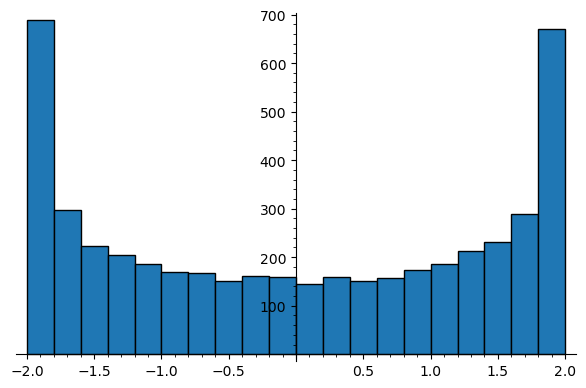
\includegraphics[height=2in]{E1.png}
	\end{center}
\end{example}
\begin{example} \label{ex:sato-tate-distribution-e2}
	Here is a histogram of the values of $a_p(E_2)$ for $p<10^5$.
	\begin{center}
		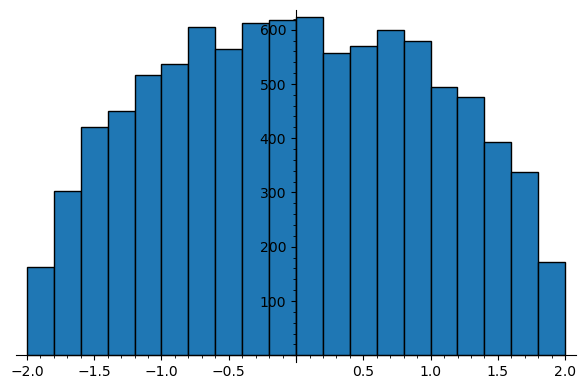
\includegraphics[height=2in]{E2.png}
	\end{center}
\end{example}
These are remarkable histograms! We encourage the reader to investigate other elliptic curves.
\begin{remark}
	It turns out that ``most of the time'' we will get a semicircle distribution as in \Cref{ex:sato-tate-distribution-e2}.
\end{remark}
A primary goal of the talk is to explain the source of these strange curves.

\subsection{The Weil Conjectures} \label{subsec:weil}
This subsection is included for motivational purposes only and can therefore be skipped without loss of too much continuity.

It will turn out that the values of $a_p(E)$ are controlled by a Galois representation attached to $E$. The most concrete way to construct this Galois representation is to use the Tate module, which we will do shortly. However, for motivation, we will state the Weil conjectures and explain how they solve our problem.
\begin{theorem}[Weil conjectures] \label{thm:weil-conj}
	Fix a smooth projective variety $X$ over a finite field $\FF_q$ of dimension $n$. Then the formal power series
	\[\zeta_X(T)\coloneqq\exp\Bigg(\sum_{r=1}^\infty\#X\left(\FF_{q^r}\right)\frac{T^r}r\Bigg)\]
	admits the following desirable properties.
	\begin{listalph}
		\item Rationality: one can write
		\[\zeta_X(T)=\frac{P_1(T)\cdots P_{2n-1}(T)}{P_2(T)\cdots P_{2n}(T)}\]
		for polynomials $P_\bullet(T)\in 1+T\ZZ[T]$.
		\item Riemann hypothesis: the roots of the polynomial $P_\bullet(T)$ are complex numbers with roots of magnitude $q^{-\bullet/2}$.
		\item Betti numbers: suppose $X$ is the reduction of a smooth projective variety $\mc X$ defined over a number ring $\OO_K$. Then $\deg P_\bullet=\dim_\CC H^\bullet(\mc X(\CC),\CC)$.
	\end{listalph}
\end{theorem}
We will not bother to explain why $\zeta_X(T)$ is the correct $\zeta$-function to look at (roughly speaking, one is supposed to plug in $T\coloneqq q^{-s}$).

The mention of Betti numbers is rather compelling because it suggests that there ought to be a way to write down a cohomology theory for smooth projective varieties $X$. Without going into too much detail, let's explain how this is done. It is possible to define a satisfactory cohomology theory called ``$\ell$-adic cohomology'' which takes as input an auxiliary prime $\ell$ which is nonzer in $\FF_q$ and then is able to (functorialy) produce cohomology groups $H^\bullet(X,\QQ_\ell)$ which are $\QQ_\ell$-vector spaces. For example, in the situation of \Cref{thm:weil-conj}(c), we find that
\[\dim_{\QQ_\ell} H^\bullet(X,\QQ_{\ell})=\dim_\CC H^\bullet(\mc X(\CC),\CC).\]
Now, for \Cref{thm:weil-conj}, the main point is to be able to compute $\#X(\FF_q)$. Well, the main idea is that $X(\FF_q)$ consists of the elements of $X(\overline{\FF_q})$ which are fixed by the Frobenius morphism $\op{Frob}_q\colon\overline{\FF_q}\to\overline{\FF_q}$. Thus, one can use the Lefschetz trace formula on our cohomology theory $H^\bullet(X,\QQ_\ell)$ to find
\[\#X(\FF_q)=\sum_{i=0}^{2d}(-1)^i\tr\left({\op{Frob}_q}\vert H^i(X,\QQ_\ell)\right).\]
Properties of the cohomology theory are then enough to prove the Weil conjectures purely formally.

For example, in the case of a curve $C$, we find that
\[\#C(\FF_q)=q+1-\tr\left({\op{Frob}_q}\vert H^1(C,\QQ_\ell)\right),\]
so we become interested in the Galois action on some $\ell$-adic vector space $H^1(C,\QQ_\ell)$. In the following section, we will provide a direct construction for (the dual of) $H^1(E,\QQ_\ell)$ for an elliptic curve $E$.
\begin{exe}
	Use the above discussion to prove \Cref{thm:hasse-weil}.
\end{exe}

\subsection{The Tate Module for Elliptic Curves} \label{subsec:tate-module-ecs}
We now go on the hunt for a Galois representation attached to $E$, where $E$ continues to be an elliptic curve defined over $\QQ$ (with a suitable integral model). It turns out that there basically one way to do this, though the recipe is somewhat roundabout. Something special about $E$ is that it comes with a group law, which means that $E(R)$ is a group (in a functorial way) for all $\QQ$-algebras $R$. For example, \Cref{ex:ec-as-c-mod-lattice} realized $E(\CC)$ as $\CC/\Lambda$ for some lattice $\Lambda$, and the group law on $\CC/\Lambda$ is the expected one.

As such, we note that $E(\overline\QQ)$ is a group with an action by $\op{Gal}(\overline\QQ/\QQ)$. One can see this purely by the ambient functoriality; alternatively, one can directly construct this action by noting that $E(\overline\QQ)\subseteq\PP^2_\QQ(\overline\QQ)$, and of course $\PP^2_\QQ(\overline\QQ)$ has a Galois action by acting on the coordinates:
\[\sigma([X:Y:Z])\coloneqq[\sigma(X):\sigma(Y):\sigma(Z)]\]
for all $\sigma\in\op{Gal}(\overline\QQ/\QQ)$ and $[X:Y:Z]\in\PP^2_\QQ(\overline\QQ)$.

However, in order to do linear algebra, we want our Galois representation to be valued in a vector space. Thus, the Galois action on $E(\overline\QQ)$ will not quite work. As such, we will want the following fact about the group law; throughout, $G[n]$ denotes the $n$-torsion of a group $G$.
\begin{proposition} \label{prop:torsion-of-ec}
	Fix an elliptic curve $E$ defined over an algebraically closed field $\overline K$. For any $n$ which is nonzero in $K$, there is a non-canonical isomorphism
	\[E(\ov K)[n]\cong(\ZZ/n\ZZ)^2.\]
\end{proposition}
\begin{example}
	For $E=\CC/\Lambda$, it is not hard to show that $E[n]$ is a group isomorphic to $(\ZZ/n\ZZ)^2$. In particular, as abstract groups, one finds that $\CC\cong\Lambda\otimes_\ZZ\RR$, so
	\[E\cong(\RR/\ZZ)^2,\]
	whose $n$-torsion has the desired property.
\end{example}
This is slightly better: for any prime $\ell$, we see that $E(\overline\QQ)[\ell]$ is a $2$-dimensional $\FF_\ell$-vector space, and more generally, $E(\overline\QQ)[\ell^\bullet)$ is a free module over $(\ZZ/\ell^\bullet\ZZ)$ of rank $2$. In order to not have to deal with torsion, we take an inverse limit.
\begin{definition}[Tate module]
	Fix an elliptic curve $E$ defined over an algebraically closed field $\overline K$. For any prime $\ell$ nonzero in $K$, we define the \textit{Tate module} as the inverse limit
	\[T_\ell E\coloneqq\limit E\left[\ell^\bullet\right],\]
	where the transition maps $E\left[\ell^{\bullet+1}\right]\onto E\left[\ell^\bullet\right]$ are given by multiplication by $\ell$. We also define $V_\ell E\coloneqq T_\ell E\otimes_\ZZ\QQ$.
\end{definition}
\begin{remark}
	We see that $T_\ell E$ is non-canonically isomorphic to $\ZZ_\ell^2$, so $V_\ell E$ is non-canonically isomorphic to $\QQ_\ell^2$.
\end{remark}
\begin{remark}
	Intuitively, one should think about $T_\ell E$ as a complex-analytic version of $H_1(E,\ZZ)$. For example, $(V_\ell E)^\lor$ should be analogous to $H^1(E,\QQ)$.
\end{remark}
The Galois action of $\op{Gal}(\overline\QQ/\QQ)$ on each $E(\overline\QQ)\left[\ell^\bullet\right]$ will now assemble into a Galois action on $T_\ell E$ and thus $V_\ell E$, so we have produced a homomorphism
\[\rho_\ell\colon\op{Gal}(\overline\QQ/\QQ)\to\op{GL}(V_\ell E).\]
It is rather difficult to compute this Galois representation directly, but it knows quite a bit about the arithmetic of $E$.
\begin{proposition} \label{prop:char-polys-on-h1}
	Fix an elliptic curve $E$ defined over a field $K$, and let $\ell$ be a prime nonzero in $K$. For any endomorphism $\varphi\colon E\to E$, let $P_\ell(T)$ be the monic characteristic polynomial of $\varphi$ acting on $V_\ell E$. For each $n\in\ZZ$, the number $P_\ell(n)$ is independent of $\ell$ and equals the degree of the map $\varphi-[n]$, where $[n]\colon E\to E$ is multiplication by $n$.
\end{proposition}
\begin{example}
	Let's compare this with what we expect to happen for $H_1(E,\ZZ)$ when $E=\CC/\Lambda$. Then $H_1(E,\ZZ)=\Lambda$, so the characteristic polynomial $P_\varphi$ of some endomorphism $\varphi\colon E\to E$ will satisfy
	\begin{align*}
		\left|P_\varphi(n)\right| &= \left|\det\left(\varphi-[n]\vert H_1(E,\ZZ)\right)\right| \\
		&= \left|\det\left(\varphi-[n]\vert \Lambda\right)\right| \\
		&= \#\left(\frac{\Lambda}{(\varphi-[n])\Lambda}\right) \\
		&= \#\left(\frac{(\varphi-[n])^{-1}\Lambda}\Lambda\right) \\
		&= \#\ker(\varphi-[n]) \\
		&= \deg(\varphi-[n]).
	\end{align*}
\end{example}
Here are two examples.
\begin{corollary} \label{cor:char-poly-frob}
	Fix an elliptic curve $E$ defined over $\QQ$ with a good enough integral model, and let $\ell$ be a prime. For a prime $p\ne\ell$, let $P_\ell(T)$ be the characteristic polynomial of $\rho_\ell({\op{Frob}_p})$, for any choice of $\op{Frob}_p$ in the conjugacy class of $\op{Gal}(\overline\QQ/\QQ)$. Then
	\[P_\ell(0)=p\qquad\text{and}\qquad P_\ell(1)=\#E(\FF_p).\]
\end{corollary}
\begin{proof}
	Let $F\colon A(\overline{\FF_p})\to A(\overline{\FF_p})$ be given by the action of $\op{Frob}_p$. \Cref{prop:char-polys-on-h1} tells us that $P_\ell(0)$ equals the degree of $F$, which is $p$ because it corresponds to the degree of some field extension which looks like $K(t^p)\subseteq K(t)$. Similarly, we see $P_\ell(1)$ equals the degree of the map $F-\id_E$, which is the number of points fixed by $F$, which is the size of $E(\FF_p)$.
\end{proof}
In particular, in the situation of the corollary, we are able to compute that
\[P_\ell(T)=T^2-aT+p,\]
where $a=(p+1)-\#E(\FF_p)$. Factoring $P_\ell(T)=(T-\alpha_{1})(T-\alpha_2)$, we find that
\[\frac1{\sqrt p}\tr\rho_\ell({\op{Frob}_p})=\frac{\alpha_1+\alpha_2}{\sqrt p}=\frac{(p+1)-\#E(\FF_p)}{\sqrt p}=a_p(E).\]
Thus, our Galois representation is good enough to understand our desired numbers $a_p(E)$!

\subsection{Defining the Sato--Tate Group: Elliptic Curves}
We continue with our elliptic curve $E$ defined $\QQ$, and we fix our auxiliary prime $\ell$. The moral of the story is that we can measure the distribution of $a_p(E)$s via the distribution of $\rho_\ell(\mathrm{Frob}_p)$; we then recover the distribution of the $a_p(E)$s by taking the trace.

Once again, we may guess that the $\rho_\ell({\mathrm{Frob}_p})$s must equidistribute in $\op{GL}(V_\ell E)\cong\op{GL}_2(\QQ_\ell)$. However, this cannot be the case because
\[\det\rho_\ell({\mathrm{Frob}_p})=p\]
by \Cref{cor:char-poly-frob}. Thus, we would like to rescale $\rho_\ell({\op{Frob}_p})$ to account for this determinant condition. Namely, we would like to replace $\rho_\ell({\mathrm{Frob}_p})$ with $\frac1{\sqrt p}\rho_\ell({\mathrm{Frob}_p})$, but there is no reasonable way to do this because $\QQ_\ell$ may not have the element $1/\sqrt p$ for all the primes $p$ we want to look at. And even when it does, there are two reasonable square roots to look at, so it is not obvious which one to choose: a different choice will lead to a different trace!

To fix this problem, we cheat: we choose any embedding $\iota\colon\QQ_\ell\into\CC$, which exists because these two fields have the same cardinality, and $\CC$ is algebraically closed. Then we may hope that the elements
\[\frac1{\sqrt p}\iota(\rho_\ell({\mathrm{Frob}_p}))\in\op{SL}_2(\CC)\]
will equidistribute as $p$ varies. However, this still cannot be the case because $\rho_\ell$ is a continuous map with compact source $\op{Gal}(\overline\QQ/\QQ)$, so these elements should actually live in some compact group. As such, we fix the compact subgroup ${\op{SU}_2}\subseteq\op{SL}_2(\CC)$, and we hope that the elements
\[\frac1{\sqrt p}\iota(\rho_\ell({\mathrm{Frob}_p}))\in{\op{SU}_2}\]
will equidistribute. Technically, this does not really make sense because $\op{Frob}_p$ was only defined up to conjugacy, so the element $\frac1{\sqrt p}\iota(\rho_\ell({\mathrm{Frob}_p}))$ will also only be defined up to conjugacy, so we are really hoping that the elements
\[\left[\frac1{\sqrt p}\iota(\rho_\ell({\mathrm{Frob}_p}))\right]\in\op{Conj}({\op{SU}_2})\]
will equidistribute.

This is generally true.
\begin{example}
	For the curve $E_2\colon y^2=x^3+x+1$, it will turn out that the conjugacy classes
	\[\left[\frac1{\sqrt p}\iota(\rho_\ell({\mathrm{Frob}_p}))\right]\in\op{Conj}({\op{SU}_2})\]
	do equidistribute in $n\op{Conj}({\op{SU}_2})$. This is the ``generic'' case for our elliptic curves, and one can show that this equidistribution gives rise to the semicircle distribution seen in \Cref{ex:sato-tate-distribution-e2} upon applying the trace.
\end{example}
In fact, one has the following.
\begin{theorem}[Sato--Tate, non-CM elliptic curve]
	Fix an elliptic curve $E$ defined over $\QQ$, and let $\ell$ be an auxiliary prime, and let $\iota\colon\QQ_\ell\to\CC$ be some embedding. Let $\rho_\ell$ be the Galois representation given by $V_\ell E$. Assume $\op{End}(E_{\overline\QQ})=\ZZ$. Then the elements
	\[\left\{\frac1{\sqrt p}\iota(\rho_\ell({\op{Frob}_p}))\right\}_{p\text{ prime}}\]
	equidistribute among the conjugacy classes of $\op{SU}_2$.
\end{theorem}
\begin{remark}
	Perhaps we ought to explain what it means to equistribute in $\op{Conj}({\op{SU}_2})$. Well, $\op{SU}_2$ is a compact topological group, so it has a Haar measure, and there is a procedure to push this measure forward along the canonical projection.
\end{remark}
The difference between \Cref{ex:sato-tate-distribution-e1,ex:sato-tate-distribution-e2} imply that we cannot expect the above discussion to be true for all elliptic curves.

To explain what is going on, note that $E_1\colon y^2=x^3+1$ has a bizarre extra endomorphism $\varphi\colon E_1\to E_1$ given by
\[\varphi(x,y)\coloneqq(\zeta_3x,y).\]
This endomorphism is defined over $\QQ(\zeta_3)$, which means that whenever ${\op{Frob}_p}\in\op{Gal}(\overline\QQ/\QQ(\zeta_3))$, we will have
\[\rho_\ell(\varphi)\circ\rho_\ell({\op{Frob}_p})=\rho_\ell({\op{Frob}_p})\circ\rho_\ell(\varphi).\]
Thus, we do not expect our elements to equidistribute in $\overline{\op{SU}_2}$: there should be an extra condition to account for commuting with endomorphisms (possibly defined over an extension of $\QQ$).

The general way to account for this is to simply ignore it. We have the following definition.
\begin{definition}[$\ell$-adic monodromy group]
	Fix an elliptic curve $E$ defined over $\QQ$, and let $\ell$ be an auxiliary prime. Let $G_\ell$ be the image of $\rho_\ell$, and let $G_\ell^{\mathrm{Zar}}$ be the smallest algebraic subgroup of $\op{GL}_{2}(\QQ_\ell)$ which is defined over $\QQ_\ell$ containining $G_\ell$. We call $G_\ell^{\mathrm{Zar}}$ the \textit{$\ell$-adic monodromy group}.
\end{definition}
We can now define the Sato--Tate group $\op{ST}(E)$ by retelling the above story.
\begin{definition}[Sato--Tate group]
	Fix an elliptic curve $E$ defined over $\QQ$, and let $\ell$ be an auxiliary prime. Let $G_\ell^{\mathrm{Zar},1}$ be the subgroup of $G_\ell^{\mathrm{Zar}}$ cut out by the condition that the determinant equals $1$. Then the \textit{Sato--Tate group} is a maximal compact subgroup of $G_\ell^{\mathrm{Zar},1}(\CC)$, where we take $\CC$-points via some embedding $\QQ_\ell\subseteq\CC$.
\end{definition}
And here is the theorem, due to Richard Taylor and many other people.
\begin{theorem}[Sato--Tate, elliptic curve] \label{thm:st-ec}
	Fix an elliptic curve $E$ defined over $\QQ$, and let $\ell$ be an auxiliary prime, and let $\iota\colon\QQ_\ell\to\CC$ be some embedding. Then the elements
	\[\left\{\frac1{\sqrt p}\iota(\rho_\ell({\op{Frob}_p}))\right\}_{p\text{ prime}}\]
	equidistribute among the conjugacy classes of $\op{ST}(E)$.
\end{theorem}
\begin{remark} \label{rem:why-in-st}
	It is not totally clear why $\frac1{\sqrt p}\iota(\rho_\ell({\op{Frob}_p}))$ would even be conjugate to any element in $\op{ST}(E)$. Roughly speaking, we are combining two properties.
	\begin{enumerate}
		\item It turns out that $\rho_\ell({\op{Frob}_p})$ is diagonalizable over an algebraic closure. Thus, our element (with eigenvalues of absolute value $1$) it certainly contained in some compact subgroup.
		\item Over $\CC$, it turns out that any compact subgroup is conjugate to a subgroup of a given maximal compact subgroup. Thus, we can conjugate our element into $\op{ST}(E)$.
	\end{enumerate}
\end{remark}
\begin{example}
	For $E_1$, one shows that $\op{ST}(E_1)$ is a normalizer of $\op U_1$ diagonally embedded in $\op{SU}_2$. Roughly speaking, the point is that the field $\QQ(\zeta_3)$ has an action on $V_\ell E_1$ which commutes with the Galois action restricted to $\op{Gal}(\overline\QQ/\QQ(\zeta_3))$, which causes the Galois action to diagonalize.
\end{example}

\subsection{The Sato--Tate Conjecture: Abelian Varieties}
In order to wrap up our story, we note that our discussion of Sato--Tate groups for elliptic curves generalizes to abelian varieties without too much effort.
\begin{definition}[abelian variety]
	Fix a field $K$. Then an \textit{abelian variety} $A$ over $K$ is a smooth projective geometrically integral group variety over $K$.
\end{definition}
Here, being a group variety means that $A(R)$ is a group (in a functorial way) for all $K$-alegbras $R$, as we had for elliptic curves.
\begin{example}
	Any product of elliptic curves continues to be an abelian variety. The category of abelian varieties is in fact abelian, so we can also take kernels and cokernels.
\end{example}
\begin{example}
	Fix a nonnegative integer $g$. Then for some lattices $\Lambda\subseteq\CC^g$, it turns out that the quotient $\CC^g/\Lambda$ is a projective variety over $\CC$, so this is an abelian variety over $\CC$ with the obvious group law.
\end{example}
Let's make explicit how the discussion of the previous two subsections generalizes to abelian varieties. Here is the generalization of \Cref{prop:torsion-of-ec}.
\begin{proposition}
	Fix an abelian vareity $A$ over a field $K$ of dimension $g$. For any $n$ which is nonzero in $K$, there is a non-canonical isomorphism
	\[E(\overline K)[n]\cong(\ZZ/n\ZZ)^{2g}.\]
\end{proposition}
This allows us to define the Tate module as before.
\begin{definition}[Tate module]
	Fix an abelian variety $A$ defined over a field $K$. For any prime $\ell$ nonzero in $K$, we define the \textit{Tate module} as the inverse limit
	\[T_\ell A\coloneqq\limit A\left[\ell^\bullet\right].\]
	We also define $V_\ell A\coloneqq T_\ell A\otimes_\ZZ\QQ$. As before, we find that $T_\ell A$ is a free module over $\ZZ_\ell$ of rank $2g$.
\end{definition}
Thus, as before, we get an $\ell$-adic Galois representation
\[\rho_\ell\colon\op{Gal}(\overline\QQ/\QQ)\to\op{GL}(V_\ell A).\]
We can also generalize some of our discussion about the characteristic polynomial. Here is the generalization of \Cref{cor:char-poly-frob}.
\begin{proposition}
	Fix an abelian variety $A$ defined over $\QQ$ with a good enough integral model, and let $\ell$ be a prime. For a prime $p\ne\ell$, let $P_\ell(T)$ be the characteristic polynomial of $\rho_\ell({\op{Frob}_p})$, for any choice of $\op{Frob}_p$ in the conjugacy class of $\op{Gal}(\overline\QQ/\QQ)$. Then $P_\ell(T)$ is a polynomial independent of $\ell$, and
	\[P_\ell(0)=p^g\qquad\text{and}\qquad P_\ell(1)=\#A(\FF_p).\]
\end{proposition}
Thus, our discussion defining $\op{ST}(E)$ can be generalized to build $\op{ST}(A)$, as follows.
\begin{enumerate}
	\item Let $G_\ell$ be the image of $\rho_\ell$ in $\op{GL}(V_\ell A)$, and let $G_\ell^{\mathrm{Zar}}$ be the smallest algebraic subgroup defined over $\QQ_\ell$ containing $G_\ell$.
	\item By choosing a Weil pairing on $T_\ell A$ (which we will not define), it turns out that there is a non-degenerate symplectic form on $V_\ell A$, and $\rho_\ell({\op{Frob}_p})$ acts with multiplier $p$ with respect to this form. Thus, we let $G_\ell^{\mathrm{Zar},1}$ be the subgroup of $G_\ell^{\mathrm{Zar}}$ cut out by preserving the corresponding symplectic form.
	\item Choose some embedding $\iota\colon\QQ_\ell\to\CC$. We now let $\op{ST}(A)$ be a maximal compact subgroup of the complex algebraic group $\iota\left(G_\ell^{\mathrm{Zar},1}\right)$.
\end{enumerate}
And here is the conjecture.
\begin{conj}[Sato--Tate] \label{conj:st}
	Fix an abelian variety $A$ defined over $\QQ$, and let $\ell$ be an auxiliary prime, and let $\iota\colon\QQ_\ell\to\CC$ be some embedding. Let $\rho_\ell$ be the Galois representation given by $V_\ell A$. Then the elements
	\[\left\{\frac1{\sqrt p}\iota(\rho_\ell({\op{Frob}_p}))\right\}_{p\text{ prime}}\]
	equidistribute among the conjugacy classes of $\op{ST}(A)$.
\end{conj}
\Cref{rem:why-in-st} once again explains why our elements have a conjugacy class in $\op{ST}(A)$. Also, note that this is a conjecture unlike \Cref{thm:st-ec}!

\subsection{Jacobian Varieties}
In order to provide some examples of abelian varieties, we introduce Jacobian varieties into our story. In order to avoid doing any difficult algebraic geometry or complex geometry, we will define these by universal property.
\begin{proposition} \label{prop:jac-up}
	Fix a curve $C$ defined over a field $K$ equipped with a point $x\in C(K)$. Then there exists an abelian variety $\op{Jac}(C)$ equipped with a map $C\into\op{Jac}(C)$ sending $x\mapsto0$ and satisfying the following the corresponding universal property: for any abelian variety $A$ and morphism $\varphi\colon C\to A$ sending $\varphi(x)=0$, there exists a unique map $\widetilde\varphi\colon\op{Jac}(C)\to A$ making the following diagram commute.
	% https://q.uiver.app/#q=WzAsMyxbMCwwLCJDIl0sWzEsMCwiXFxvcHtKYWN9KEMpIl0sWzEsMSwiQSJdLFswLDIsIlxcdmFycGhpIiwyXSxbMSwyLCJcXHdpZGV0aWxkZVxcdmFycGhpIiwwLHsic3R5bGUiOnsiYm9keSI6eyJuYW1lIjoiZGFzaGVkIn19fV0sWzAsMSwiIiwwLHsic3R5bGUiOnsidGFpbCI6eyJuYW1lIjoiaG9vayIsInNpZGUiOiJ0b3AifX19XV0=&macro_url=https%3A%2F%2Fraw.githubusercontent.com%2FdFoiler%2Fnotes%2Fmaster%2Fnir.tex
	\[\begin{tikzcd}
		C & {\op{Jac}(C)} \\
		& A
		\arrow[hook, from=1-1, to=1-2]
		\arrow["\varphi"', from=1-1, to=2-2]
		\arrow["{\widetilde\varphi}", dashed, from=1-2, to=2-2]
	\end{tikzcd}\]
\end{proposition}
\begin{definition}[Jacobian]
	Fix a curve $C$ defined over a field $K$ equipped with a point $x\in C(K)$. Then the abelian variety $\op{Jac}(C)$ produced by \Cref{prop:jac-up} is called the \textit{Jacobian} of $C$.
\end{definition}
\begin{example}
	For an elliptic curve $E$, we see that $\op{Jac}(E)=E$ because $E$ is already an abelian variety.
\end{example}
\begin{example}
	Let's give the construction for $\op{Jac}(C)$ when our curve $C$ is defined over $\CC$. One can embed the first homology $H_1(C,\ZZ)$ into the complex vector space $H^0(C,\Omega^1_C)^\lor$ by taking $[\gamma]\in H_1(C,\ZZ)$ to the functional
	\[\omega\mapsto\int_\gamma\omega.\]
	Then $\op{Jac}(C)=H^0(C,\Omega^1_C)^\lor/H_1(C,\ZZ)$.
\end{example}
\begin{remark}
	It is not obvious from the definition, but it turns out that the dimension of $\op{Jac}(C)$ equals the genus of the curve $C$.
\end{remark}
\begin{remark}
	Motivated by \cref{subsec:weil}, the importance of the Jacobian arises from the fact that the map $C\to\op{Jac}(C)$ induces an isomorphism
	\[H^1(\op{Jac}(C),\QQ_\ell)\to H^1(C,\QQ_\ell)\]
	on first cohomology. In particular, we can hope to read off properties of the curve (related to its cohomology) from the Jacobian. The analogous statement for $\CC$ is simply that $H_1(C,\ZZ)\to H_1(\op{Jac}(C),\ZZ)$ is an isomorphism, which is clear from our construction.
\end{remark}
The following result follows from the discussion in \cref{subsec:weil} and the above remark.
\begin{proposition}
	Fix a curve $C$ defined over $\QQ$ with a good enough integral model, and set $A\coloneqq\op{Jac}(C)$. For any prime $p$ and an auxiliary prime $\ell\ne p$, we have
	\[\#C(\FF_p)-(p+1)=\tr\left(\rho_\ell({\op{Frob}_p})\vert V_\ell A\right)\]
\end{proposition}
Thus, we expect computable (but perhaps complicated) equidistribution results for general curves to follow from \Cref{conj:st}. Here is one such histogram.
\begin{example}
	Consider the genus-$2$ curve $C\colon y^2=x^5+x+1$. Here is a histogram for the values of $a_p(C)\coloneqq(\#C(\FF_p)-(p+1))/\sqrt p$ for $p<10^5$.
	\begin{center}
		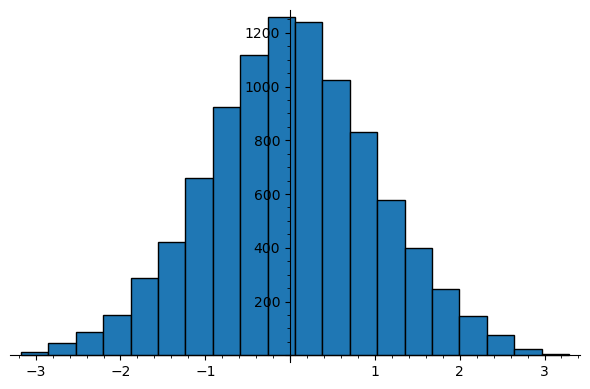
\includegraphics[height=2in]{hyper.png}
	\end{center}
\end{example}

\end{document}